\documentclass[../main.tex]{subfiles}

\begin{document}


%
% -----------------------------------------------------------------------------------------------------------------
%

\begin{frame}[t]{Assumptions}
\begin{itemize}
\item \textbf{Assumption} Smart meter measurements are considered time synchronised with respect to system changes, i.e. for the $m$-th measurement taken from every node, load impedances remain constant.
	\begin{figure}[H]
	  \centering
	  \begin{tikzpicture}
	    \coordinate (zero) at (0, 0);
	    \coordinate (node_n) at (8, 0);
	    \coordinate (tn) at (0, 2);
	    \coordinate (g0) at (0, 0.5);
	    \coordinate (g1) at (0, 1.5);
	    \coordinate (g2) at (8, 1.5);
	    \coordinate (g3) at (8, 0.5);
	    \draw[dotted, thin, fill=gray!20] (g0)--(g1)--node[above]{Single measurement timespan}(g2)--(g3)--(g0);
	    \draw[arrows = {-Stealth[inset=0pt, angle=25:5pt]}] (zero) -- (node_n) node[above right]{Node number};
	    \draw[arrows = {-Stealth[inset=0pt, angle=25:5pt]}] (zero) -- (tn) node[left]{$t$};

	    % dot coordinates
	    \coordinate (d0) at (1, 0.7);
	    \coordinate (d0p) at (1, 0);
	    \coordinate (d1) at (2, 1.3);
	    \coordinate (d1p) at (2, 0);
	    \coordinate (d2) at (3, 1.1);
	    \coordinate (d2p) at (3, 0);
	    \coordinate (d3) at (4, 1.2);
	    \coordinate (d3p) at (4, 0);
	    \coordinate (d4) at (6, 1.3);
	    \coordinate (d4p) at (6, 0);
	    \coordinate (d5) at (7, 0.9);
	    \coordinate (d5p) at (7, 0);

	    \draw[fill] (d0) circle [radius=0.1]; \draw[dotted] (d0) -- (d0p)node[below]{$1$};
	    \draw[fill] (d1) circle [radius=0.1]; \draw[dotted] (d1) -- (d1p)node[below]{$2$};
	    \draw[fill] (d2) circle [radius=0.1]; \draw[dotted] (d2) -- (d2p)node[below]{$3$};
	    \draw[fill] (d3) circle [radius=0.1]; \draw[dotted] (d3) -- (d3p)node[below]{$4$};
	    \draw[fill] (d4) circle [radius=0.1]; \draw[dotted] (d4) -- (d4p)node[below]{$N-1$};
	    \draw[fill] (d5) circle [radius=0.1]; \draw[dotted] (d5) -- (d5p)node[below]{$N$};
	  \end{tikzpicture}
	  %\caption{Time synchronicity assumption. Gray region is a single time stamp corresponding to $m$-th measurement.}
	\end{figure}
	% \item<2-> \textbf{Justification} Smart metering minimum functionality specifications (in Australia) require smart meters to maintain measurement time clocks to within a few seconds across a network \cite{NMI_au}.
\end{itemize}

% \uncover<3->{
% \textbf{Note}: 
% 	\begin{itemize}
% 		\item We do not assume PMU availability \cite{han2016automated}
% 	\end{itemize}	
% }
	
\setbeamercolor{alerted text}{fg=black ,bg=yellow}
\end{frame}


%
% -----------------------------------------------------------------------------------------------------------------
%





%
% -----------------------------------------------------------------------------------------------------------------
%



\begin{frame}[t]{Optimisation problem}

\begin{columns}
	\colorbox{gray!20}{\begin{column}{0.5\textwidth}
		\textbf{Backward model}
		\begin{equation*}
		  \begin{split}
		  v_{n-1}e^{i\Delta_{n}} - v_{n} = j_{n}z_{n}, \\
		  j_{n-1} = i_{n-1} + j_{n}e^{-i\Delta_{n}}
		  \end{split}
		\end{equation*}
	\end{column}}
	\begin{column}{0.5\textwidth}
		%\begin{figure}[H]
		\begin{tikzpicture}
			\draw[thin, dotted] (-2, 0) -- (0, 0);
			\draw[arrows = {-Stealth[inset=0pt, angle=30:10pt]}, dotted] (-2, 0) -- (-0.5,0)  node[below left]{$j_{n-1}$};
			\draw[fill] (0,0) circle [radius=0.1] node[above, black]{$v_{n-1}$};
			\draw[arrows = {-Stealth[fill=none, inset=0pt, angle=90:10pt]}, thick] (0,0) -- node[right]{$i_{n-1}$}(0, -1);
			\draw[thick] (0,0) -- (4,0);
			\draw[arrows = {-Stealth[inset=0pt, angle=30:10pt]}, thick] (0, 0) -- (1.5,0)  node[below]{$j_{n}$};
			\draw[fill] (4,0) circle [radius=0.1] node[above]{$v_{n}$};
			\draw[arrows = {-Stealth[fill=none, inset=0pt, angle=90:10pt]}, thick] (4, 0) -- node[right]{$i_{n}$}(4, -1);

			\coordinate (a) at (-1, -1.5);
			\coordinate (b) at (1, -1.5);
			\coordinate (c) at (0.9, -1.1);

			\draw[dotted] (a) -- node[below right]{$\Delta_{n}$} (b);
			\draw[arrows = {-Stealth[inset=0pt, angle=30:10pt]}] (a) -- (c) node[below right]{$v_{n-1}$};
			\pic[draw,-,angle eccentricity=1.35, angle radius=1.4cm, thick] {angle=b--a--c};
			%\pic[draw,-,angle eccentricity=1.15, angle radius=1.5cm, red, ultra thick] {angle=c--a--b};
			%\draw[arrows = {-Stealth[inset=0pt, angle=30:10pt]}] (a) -- (d) node[midway, below]{$i_1$};
			%\pic["$\theta_1$", draw,-,angle eccentricity=1.4, angle radius=1cm] {angle=d--a--c};
			%\pic[draw,-,angle eccentricity=1.15, angle radius=0.5cm, red, ultra thick] {angle=d--a--b};

			\coordinate (a1) at (3, -1.5);
			\coordinate (b1) at (5, -1.5);
			\coordinate (c_shifted) at (4.9, -1.8);
			\coordinate (c1) at (4.6, -2.4);

			%\draw[dotted] (a1) -- (b1);
			%\draw[arrows = {-Stealth[inset=0pt, angle=30:10pt]}, dashed] (a1) -- (c_shifted) node[right]{$v_{n-1}$};
			\draw[arrows = {-Stealth[inset=0pt, angle=30:10pt]}] (a1) -- (b1) node[below right]{$v_n$};
			%\pic["$\Delta_{n}$", draw,-,angle eccentricity=1.35, angle radius=1.4cm, thick] {angle=c1--a1--c_shifted};

		\end{tikzpicture}
		%\end{figure}
	\end{column}
\end{columns}

\uncover<2->{
	for each power line we solve:

	% \begin{equation*}
	\begin{align}
	& \min_{\bm{z}, \bm{\gamma}} \Big\| \bm{V}_{n-1}\bm{\gamma} - |\bm{v}_{n}| - \bm{J}\bm{z} \Big\|_2^2 & \quad \text{\textcolor{gray}{(real part of the first equation)}} \nonumber \\
	& \st ~ \gamma^{(m)} = \sqrt{1 - \frac{( \bm{j}^{(m)}\mathcal{Q}\bm{z} )^2}{|v^{(m)}_{n-1}|^2} }, ~m=1, & \ldots, M \quad \text{\textcolor{gray}{(imag part of the first equation)}} \nonumber
	\end{align}
	% \end{equation*}
}

\uncover<3->{
	\begin{itemize}
	\item $\bm{\gamma}$ - phase angle parameter $\in (0, 1)$, $\bm{J}$ - matrix of line currents, $\bm{V}_n = \diag{(|\bm{v}_{n}|)}$
	\item problem is non-convex and non-linear
	\end{itemize}	
}

\end{frame}



%
% -----------------------------------------------------------------------------------------------------------------
%



% \begin{frame}[t]{Developed approach}
% \begin{columns}
% \colorbox{gray!20}{\begin{column}{0.5\textwidth}

% \textbf{Problem}:
% \begin{equation*}
% \min_{\bm{z}, \bm{\gamma}} f(\bm{z}, \bm{\gamma}), \quad \st \bm{\gamma} = \bm{g}(\bm{z})
% \end{equation*}
% \textbf{Idea}: find roots of 
% $$\bm{\gamma} = \bm{g}(\argmin_{\bm{z}} f(\bm{z}, \bm{\gamma})) = \bm{\phi}(\bm{\gamma})$$
% \textbf{Iteration}:
% \begin{equation*}
% \begin{split}
% &{} \bm{\gamma}^{(0)} = \bm{1} \\
% & \bm{\gamma}^{(i+1)} = \bm{\gamma}^{(i)} + \alpha \Big[\bm{\phi}(\bm{\gamma}^{(i)}) - \bm{\gamma}^{(i)}\Big]
% \end{split}
% \end{equation*}

% \end{column}}


% \begin{column}{0.5\textwidth}
% Details:
% \begin{equation*}
% \begin{split}
% & f(\bm{z}, \bm{\gamma}) = \Big\| \bm{V}_n\bm{\gamma} - |\bm{v}_{n+1}| - \bm{J}\bm{z} \Big\|_2^2 \\
% & \gamma^{(m)} = \sqrt{1 - \frac{( \bm{j}^{(m)}\mathcal{Q}\bm{z} )^2}{|v^{(m)}_n|^2} } = g^{(m)}(\bm{z})
% \end{split}
% \end{equation*}
% \begin{itemize}
% \item $\bm{\gamma}$ - phase angle parameter $\in [0, 1]$, 
% \item $\bm{J}$ - matrix of line currents 
% \item $|\bm{v}_n|$ - RMS voltage measurements at node $n$, $\bm{V}_n = \diag{(|\bm{v}_{n}|)}$
% \end{itemize}

% \end{column}
% \end{columns}

% \begin{itemize}
% 	\item $i = 0$ corresponds to a linearised case, i.e. phase increments between nodes are ignored.
% 	\item Next iterations concurrently improve estimation
% \end{itemize}

% \end{frame}



%
% -----------------------------------------------------------------------------------------------------------------
%



\begin{frame}[t]{Developed approach}
\begin{columns}
\colorbox{gray!20}{\begin{column}{0.5\textwidth}

\textbf{Problem}:
\begin{equation*}
\min_{\bm{x}, \bm{y}} \underbrace{\|A\bm{x} + B\bm{y} + \bm{c}\|}_{f(\bm{x}, \bm{y})}, \quad \st \bm{y} = \bm{g}(\bm{x})
\end{equation*}
\textbf{Idea}: if $A, B$ - full rank and $\bm{g}$ is differentiable and surjective, find roots of 
$$\bm{y} = \bm{g}(\argmin_{\bm{x}} f(\bm{x}, \bm{y})) = \bm{\phi}(\bm{y})$$
\end{column}}


\begin{column}{0.5\textwidth}
\begin{equation*}
\begin{split}
& f(\bm{z}, \bm{\gamma}) = \Big\| \bm{V}_{n-1}\bm{\gamma} - |\bm{v}_{n}| - \bm{J}\bm{z} \Big\|_2^2 \\
& \gamma^{(m)} = \sqrt{1 - \frac{( \bm{j}^{(m)}\mathcal{Q}\bm{z} )^2}{|v^{(m)}_{n-1}|^2} } = g^{(m)}(\bm{z})
\end{split}
\end{equation*}

\begin{itemize}
		\item $\bm{V}_{n-1}, \bm{J}$ are full rank
		\item $g^{(m)}$ is differentiable, surjective function for each $m$
	\end{itemize}

\end{column}
\end{columns}

\uncover<2->{
	\begin{columns}
	\colorbox{gray!20}{\begin{column}{0.5\textwidth}

	\textbf{Iteration}:
	\begin{equation*}
	\begin{split}
	&{} \bm{\gamma}^{(0)} = \bm{1} \\
	& \bm{\gamma}^{(i+1)} = \bm{\gamma}^{(i)} + \alpha \Big[\bm{\phi}(\bm{\gamma}^{(i)}) - \bm{\gamma}^{(i)}\Big]
	\end{split}
	\end{equation*}
	\end{column}}


	\begin{column}{0.5\textwidth}
	\begin{itemize}
		\item $i = 0$ corresponds to a linearised case, i.e. phase increments between nodes are ignored.
		\item Next iterations concurrently improve estimation
	\end{itemize}
	\end{column}
	\end{columns}
	
}
\end{frame}


%
% -----------------------------------------------------------------------------------------------------------------
%


\begin{frame}[t]{Developed approach. Estimation results}

\begin{columns}[t]
\begin{column}{0.4\textwidth}
\centering
\begin{itemize}
\only<1-2>{
\item Feeder type: linear
\item Number of loads: 10
\item Load parameters: 
	\begin{itemize}
	 	\item European LV Test Feeder
	 \end{itemize} 
% \item Measurement noise: 
% 	\begin{itemize}
% 		\item Gaussian
% 		\item Full scale
% 	\end{itemize}
}
% \only<3->{
% \item Linear feeder
% \item 10 loads
% \item European LV Test Feeder
% \item Noise: 
% 	\begin{itemize}
% 		\item Gaussian
% 		\item Full scale
% 	\end{itemize}
% \item Computation time: $\le$ \textbf{1s}
% \item Result:
% \begin{itemize}
% 	\item 1\% FS error: \textcolor{red}{~50\%} estimation error
% 	\item 0.5\% FS error: \textcolor{blue}{~15\%} estimation error
% 	\item 0.1\% FS error: \textcolor{black}{~5\%} estimation error
% \end{itemize}
% }
\end{itemize}

% \uncover<2->
% {
% \begin{enumerate}
% \item Relative error is less than \textbf{30\%.} with \textbf{1\%} measurement noise.
% \item Computation time: $\mathbf{\le 1 s.}$
% \end{enumerate}
% }

\end{column}

\begin{column}{0.6\textwidth}
\centering
\only<2>
	{
		Noise free:
			\centering
			\begin{adjustbox}{width=1\columnwidth}
			\input{pics/z_rel_err_bci_.tex}
			\end{adjustbox}
	}

% \only<3>
% 	{
% 		Noise added:
% 			\centering
% 			\begin{adjustbox}{width=1\columnwidth}
% 			% This file was created by matlab2tikz.
%
%The latest updates can be retrieved from
%  http://www.mathworks.com/matlabcentral/fileexchange/22022-matlab2tikz-matlab2tikz
%where you can also make suggestions and rate matlab2tikz.
%
% \documentclass[tikz]{standalone}
% \usepackage[T1]{fontenc}
% \usepackage[utf8]{inputenc}
% \usepackage{pgfplots}
% \usepackage{grffile}
% \pgfplotsset{compat=newest}
% \usetikzlibrary{plotmarks}
% \usepgfplotslibrary{patchplots}
% \usepackage{amsmath}

% \begin{document}
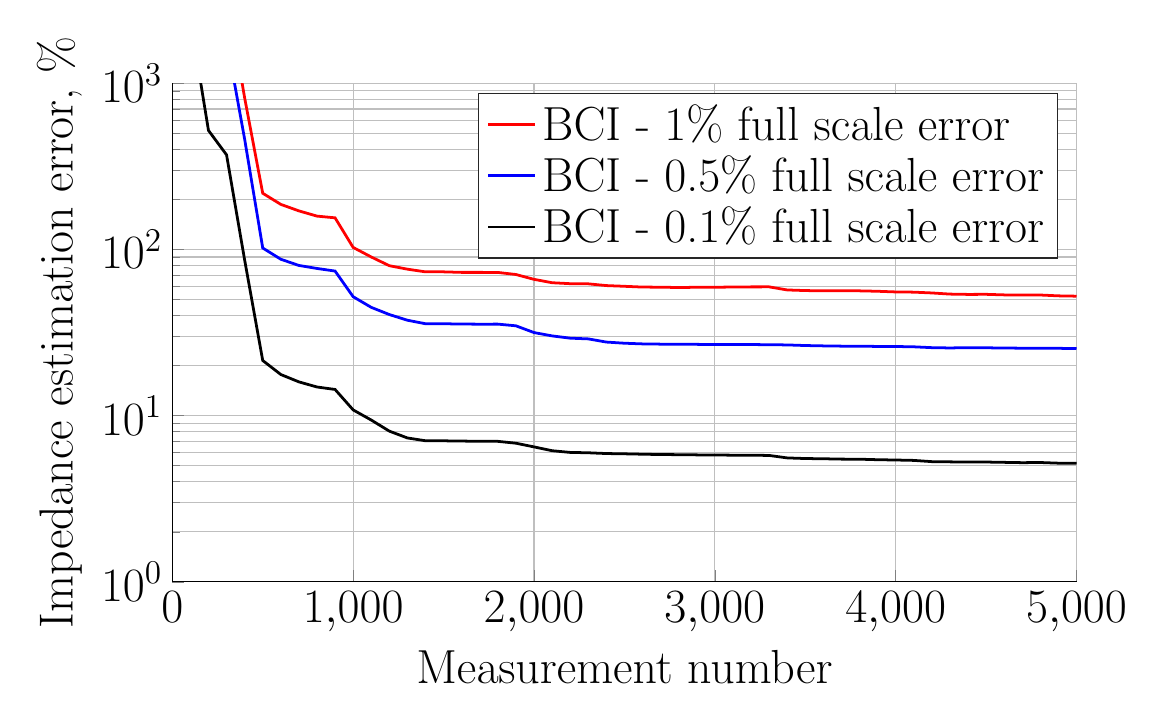
\begin{tikzpicture}

\begin{axis}[%
width=4.521in,
height=2.493in,
at={(0.758in,0.434in)},
scale only axis,
xmin=0,
xmax=5000,
xtick={   0, 1000, 2000, 3000, 4000, 5000},
xlabel={Measurement number},
xmajorgrids,
ymode=log,
ymin=1,
ymax=1000,
yminorticks=true,
% ylabel={$\frac{\|\mathbf{z} - \hat{\mathbf{z}}\|_2}{\|\mathbf{z}\|_2}$, \%},
ylabel={Impedance estimation error, \%},
ymajorgrids,
yminorgrids,
axis background/.style={fill=white},
axis x line*=bottom,
axis y line*=left,
%legend style={at={(0.5,1.03)},anchor=south,legend cell align=left,align=left,draw=white!15!black},
legend style={legend cell align=left, align=right, draw=white!15!black},
xlabel style={font=\LARGE},ylabel style={font=\LARGE},legend style={font=\LARGE},ticklabel style={font=\LARGE}
]
\addplot [color=red,solid,line width=1.0pt]
  table[row sep=crcr]{%
100	22728.0844401917\\
200	5118.69657000351\\
300	3536.99850914306\\
400	816.769790166386\\
500	217.789962578717\\
600	186.673358272156\\
700	170.588712436484\\
800	158.672266693795\\
900	154.945990194417\\
1000	102.812960987144\\
1100	90.0903675033844\\
1200	79.8235730543928\\
1300	76.0952811801202\\
1400	73.2939001233863\\
1500	73.3105008058256\\
1600	72.7745763727444\\
1700	72.7783815896182\\
1800	72.718031543639\\
1900	70.6605592162223\\
2000	66.0800688049927\\
2100	63.0546347055478\\
2200	62.2194878973759\\
2300	62.0956124039623\\
2400	60.6097719919569\\
2500	60.0059486729373\\
2600	59.3725361804331\\
2700	59.273596157382\\
2800	58.9970650417395\\
2900	59.2004854022767\\
3000	59.2540643803915\\
3100	59.3824432036232\\
3200	59.5270961745916\\
3300	59.5457679559992\\
3400	57.0456483739896\\
3500	56.5590202126003\\
3600	56.3618548265959\\
3700	56.3310515498867\\
3800	56.3326145456274\\
3900	56.0118499285963\\
4000	55.4987848173866\\
4100	55.3352463267593\\
4200	54.7210962583346\\
4300	53.8589408369959\\
4400	53.6297037181513\\
4500	53.6839536356162\\
4600	53.2751694592901\\
4700	53.2522253135632\\
4800	53.177736128386\\
4900	52.5670815106881\\
5000	52.3268073688193\\
};
\addlegendentry{BCI - 1\% full scale error};

\addplot [color=blue,solid,line width=1.0pt]
  table[row sep=crcr]{%
100	11400.6317104915\\
200	2709.11003762981\\
300	1837.480807797\\
400	460.735052239631\\
500	102.005394167206\\
600	87.2906130185545\\
700	80.0915493937165\\
800	76.8472619532403\\
900	74.1173835937968\\
1000	51.9491088048463\\
1100	44.8245611687652\\
1200	40.5784875779692\\
1300	37.5024040866603\\
1400	35.7216733221953\\
1500	35.7193452101075\\
1600	35.5593681721333\\
1700	35.5168223438536\\
1800	35.5311590526479\\
1900	34.7140095542001\\
2000	31.6135326665586\\
2100	30.1820496229043\\
2200	29.251150624789\\
2300	28.9584491275208\\
2400	27.7120685560186\\
2500	27.2715114539494\\
2600	27.0170947009927\\
2700	26.9242291975569\\
2800	26.8678826767531\\
2900	26.8440375438859\\
3000	26.772186808124\\
3100	26.7609659888137\\
3200	26.7669739770353\\
3300	26.7189769781261\\
3400	26.6314209655037\\
3500	26.4145706764439\\
3600	26.281180847016\\
3700	26.18937750428\\
3800	26.1581314055083\\
3900	26.086201997588\\
4000	26.0601240884831\\
4100	25.9459986670809\\
4200	25.6442362748963\\
4300	25.5423909233786\\
4400	25.6431195654694\\
4500	25.5931984861965\\
4600	25.5147322817117\\
4700	25.4599795184458\\
4800	25.4167488602764\\
4900	25.4113724076065\\
5000	25.3137359321453\\
};
\addlegendentry{BCI - 0.5\% full scale error};

\addplot [color=black,solid,line width=1.0pt]
  table[row sep=crcr]{%
100	2426.97935227751\\
200	520.097429495387\\
300	370.627433664178\\
400	86.4088147076159\\
500	21.4660738897338\\
600	17.6791178477347\\
700	15.9634979839217\\
800	14.8705928411826\\
900	14.3726130409558\\
1000	10.8271106697378\\
1100	9.40872402129834\\
1200	8.06864024640509\\
1300	7.34031789104499\\
1400	7.06138614146183\\
1500	7.05484216150573\\
1600	7.0294981712566\\
1700	7.01212772537375\\
1800	7.00416054756797\\
1900	6.82498779889169\\
2000	6.48510124758661\\
2100	6.15065684701161\\
2200	6.00827285737952\\
2300	5.97754929288951\\
2400	5.9144943049684\\
2500	5.89186642858549\\
2600	5.85979970044402\\
2700	5.83257088974041\\
2800	5.82381641579081\\
2900	5.8059225153119\\
3000	5.79328015943364\\
3100	5.78378652643428\\
3200	5.778141003319\\
3300	5.76138406166361\\
3400	5.56721982716132\\
3500	5.51920557437916\\
3600	5.50204025657614\\
3700	5.47477625359662\\
3800	5.46857327003434\\
3900	5.43009535981615\\
4000	5.40738490087627\\
4100	5.37831097108823\\
4200	5.28639416421409\\
4300	5.27038746815866\\
4400	5.2594982138701\\
4500	5.25765191351608\\
4600	5.23462274053984\\
4700	5.2121104596335\\
4800	5.22313758218916\\
4900	5.1755789476994\\
5000	5.1637319100943\\
};
\addlegendentry{BCI - 0.1\% full scale error};

\end{axis}
\end{tikzpicture}%
% \end{document}
% 			\end{adjustbox}
% 	}

\end{column}

\end{columns}

\only<2>
{
	\textbf{Note}:
	\begin{itemize}
		\item \textbf{BCI} after 1 iteration is equivalent to conventional methods
	\end{itemize}	
}

\end{frame}


%
% -----------------------------------------------------------------------------------------------------------------
%


\begin{frame}[t]{Iteration interpretation}
\begin{columns}[T]
\begin{column}{0.5\textwidth}

  \begin{figure}[t]
  \centering
  \begin{tikzpicture}
  \begin{axis}[xmin=0,xmax=1,
              ymin=0,ymax=1,
              grid=both,
              grid style={line width=.1pt, draw=gray!10},
              major grid style={line width=.2pt,draw=gray!50},
              axis lines=middle,
              minor tick num=4,
              enlargelimits={abs=0.2},
              axis line style={latex-latex},
              ticklabel style={font=\tiny, fill=white},
              xlabel style={at={(ticklabel* cs:1)},anchor=north west},
              ylabel style={at={(ticklabel* cs:1)},anchor=south west},
              xlabel = {$~\gamma_1$},
              ylabel = {$\gamma_2$}]
  \addplot[name path=F,black!,domain={0:1}, samples=101] {sqrt(1 - 0.02*(12*x - 6)^2)} node[pos=0.6, above left]{$\phi$};
  %Sqrt[1 - 0.0000135558 (-200 + 220 x)^2] mathematica approximate result
  \addplot[name path=G,black,domain={-1:2}] {x};
  \addplot[pattern=north west lines, pattern color=red!50]fill between[of=F and G, soft clip={domain=0.82:1}];
  \node[label={90:{$\gamma^{(0)}$}},circle,fill,inner sep=1pt] at (axis cs:1,1) {};
  \node[label={90:{$\gamma^*$}},circle,fill,inner sep=1pt] at (axis cs:0.827,0.827) {};
  \end{axis}
  \end{tikzpicture}
  \end{figure}

\end{column}



\begin{column}{0.5\textwidth}
	\textbf{Observation:}
	\begin{equation*}
	\bm{\gamma}^{(i+1)} = \bm{\gamma}^{(i)} + \alpha \Big[\bm{\phi}(\bm{\gamma}^{(i)}) - \bm{\gamma}^{(i)}\Big]
	\end{equation*} - is a gradient ascent iteration for 

	\begin{equation*}
		\int_{\bm{\gamma}^{(0)}}^{\bm{\gamma}} \big[\bm{\phi}(\bm{\bar{\gamma}}) - \bm{\bar{\gamma}}\big] d \bm{\bar{\gamma}}	
	\end{equation*}

	i.e. this iteration maximises the \textbf{area} shown in red.


\end{column}
\end{columns}
\end{frame}


%
% -----------------------------------------------------------------------------------------------------------------
%


\begin{frame}[t]{Modifications}
\begin{itemize}
	\item Prior knowledge of cable parameters
	
	\textbf{Idea:} known $X/R$ ration of cables reduces condition number of the optimisation problem

	\item Decentralised calculations

	\textbf{Idea:} Every smart meter can calculate the impedance between itself and its neighbour.
	\begin{columns}
	\begin{column}{0.5\linewidth}
	\centering
	\begin{tikzpicture}
	\uncover<6->{\path[->, >=stealth, dotted] (3.9,0.1) edge[bend right = 45] (2.1,0.1);}
	\uncover<4->{\path[->, >=stealth, dotted] (5.9,0.1) edge[bend right = 45] (4.1,0.1);}
	\uncover<2->{\path[->, >=stealth, dotted] (7.9,0.1) edge[bend right = 45] (6.1,0.1);}

	\draw[arrows = {-Stealth[fill=none, inset=0pt, angle=90:10pt]}, thick] (2,0) -- (2,-1);
	\draw[arrows = {-Stealth[fill=none, inset=0pt, angle=90:10pt]}, thick] (4,0) -- (4,-1);
	\draw[arrows = {-Stealth[fill=none, inset=0pt, angle=90:10pt]}, thick] (6,0) -- (6,-1);
	\draw[arrows = {-Stealth[fill=none, inset=0pt, angle=90:10pt]}, thick] (8,0) -- (8,-1);

	\only<1-7>
	{
	\draw[thick, dotted, red] (1.5,0) -- (2,0);
	%\draw[fill,red] (2,0) circle [radius=0.1];
	}
	\only<8->
	{
	\draw[thick] (1.5,0) -- (2,0);
	%\draw[fill] (2,0) circle [radius=0.1];
	}
	\only<1-6>
	{
	\draw[thick, red] (2,0) -- (4,0);
	\draw[fill,red] (2,0) circle [radius=0.1];
	}
	\only<7->
	{
	\draw[thick] (2,0) -- (4,0);
	\draw[fill] (2,0) circle [radius=0.1];
	}
	\only<1-4>
	{
	\draw[thick, red] (4,0) -- (6,0);
	\draw[fill,red] (4,0) circle [radius=0.1];
	}
	\only<5->
	{
	\draw[thick] (4,0) -- (6,0);
	\draw[fill] (4,0) circle [radius=0.1];
	}
	\only<1-2>
	{
	\draw[thick, red] (6,0) -- (8,0);
	\draw[fill, red] (6,0) circle [radius=0.1];
	}
	\only<3->
	{
	\draw[thick] (6,0) -- (8,0);
	\draw[fill] (6,0) circle [radius=0.1];
	}
	\draw[fill] (8,0) circle [radius=0.1];
	\end{tikzpicture}
	\end{column}
	\begin{column}{0.5\linewidth}
	% \begin{minipage}[t][.6\textheight][c]{\linewidth}
	\centering
	\begin{tikzpicture}
	\draw[dotted, thick] (0.5,0) -- (1,0);
	\node at (4,0) [rectangle,draw] (SM_n) {$\mathbf{SM}_{n}$};
	\draw[thick] (1,0) -- (SM_n);
	%\draw (4,0) circle [radius=1] node[above right]{$n$};
	\draw[thick] (1,0) -- (2, 0) node[above, red]{$z_{n-1}$};
	\draw[thick] (SM_n) -- (7,0);
	\draw[dotted, thick] (7,0) -- (7.5,0);
	\draw[thick] (SM_n) -- (6,0) node[above]{$z_{n}$};
	\draw[arrows = {-Stealth[fill=none, inset=0pt, angle=90:10pt]}, thick] (SM_n) -- (4,-1);
	\draw (1,1) -- (3,1) -- (SM_n);
	\draw[arrows = {-Stealth[inset=0pt, angle=30:10pt]}] (3, 1) -- (2, 1) node[above]{data to $\mathbf{SM}_{n-1}$};
	\draw (SM_n) -- (5,1) -- (7,1);
	\draw[arrows = {-Stealth[inset=0pt, angle=30:10pt]}] (7, 1) -- (6, 1) node[above]{data from $\mathbf{SM}_{n+1}$};
	%\draw (SM_n) -- (5,-1) -- (7,-1) node[pos = 1/2, below]{$z_{n}$};
	\end{tikzpicture}
	% \end{minipage}
	\end{column}
	\end{columns}
	\textbf{Requirements:} 
	\begin{itemize}
	\item Communication between every neighbouring pair of smart meters;
	\end{itemize}

\end{itemize}
\end{frame}



\begin{frame}[t]{Simulation results}

\begin{columns}[t]
\begin{column}{0.3\textwidth}
\centering

\begin{itemize}
\only<1>{
\item Feeder type: linear
\item Number of loads: 10
\item Load parameters: 
	\begin{itemize}
	 	\item European LV Test Feeder data
	 \end{itemize} 
\item Measurement noise: 
	\begin{itemize}
		\item Gaussian
		\item Full scale
	\end{itemize}
\item Algorithms:
	\begin{itemize}
		\item BCI - original
		\item DBCI$_{XR}$ - with 
		modifications
	\end{itemize}
}
\only<2->{
\item Linear feeder
\item 10 loads
\item European LV Test Feeder data
\item Noise: 
	\begin{itemize}
		\item Gaussian
		\item Full scale
	\end{itemize}
\item Algorithms:
	\begin{itemize}
		\item BCI - original
		\item DBCI$_{XR}$ - with 
		modifications
	\end{itemize}
}
\end{itemize}

% \uncover<2->
% {
% \begin{enumerate}
% \item Relative error is less than \textbf{30\%.} with \textbf{1\%} measurement noise.
% \item Computation time: $\mathbf{\le 1 s.}$
% \end{enumerate}
% }

\end{column}

\begin{column}{0.7\textwidth}
\centering
\uncover<2->
	{
		Noise free:
		\begin{columns}[t]
		\begin{column}{0.55\textwidth}
			\centering
			\begin{adjustbox}{width=1\columnwidth}
			\input{pics/z_rel_err_bci_.tex}
			\end{adjustbox}
		\end{column}
		\begin{column}{0.55\textwidth}
			\centering
			\begin{adjustbox}{width=1\columnwidth}
			\input{pics/z_rel_err_.tex}
			\end{adjustbox}
		\end{column}
		\end{columns}
		Noise added:
		\begin{columns}[t]
		\begin{column}{0.55\textwidth}
			\centering
			\begin{adjustbox}{width=1\columnwidth}
			% This file was created by matlab2tikz.
%
%The latest updates can be retrieved from
%  http://www.mathworks.com/matlabcentral/fileexchange/22022-matlab2tikz-matlab2tikz
%where you can also make suggestions and rate matlab2tikz.
%
% \documentclass[tikz]{standalone}
% \usepackage[T1]{fontenc}
% \usepackage[utf8]{inputenc}
% \usepackage{pgfplots}
% \usepackage{grffile}
% \pgfplotsset{compat=newest}
% \usetikzlibrary{plotmarks}
% \usepgfplotslibrary{patchplots}
% \usepackage{amsmath}

% \begin{document}
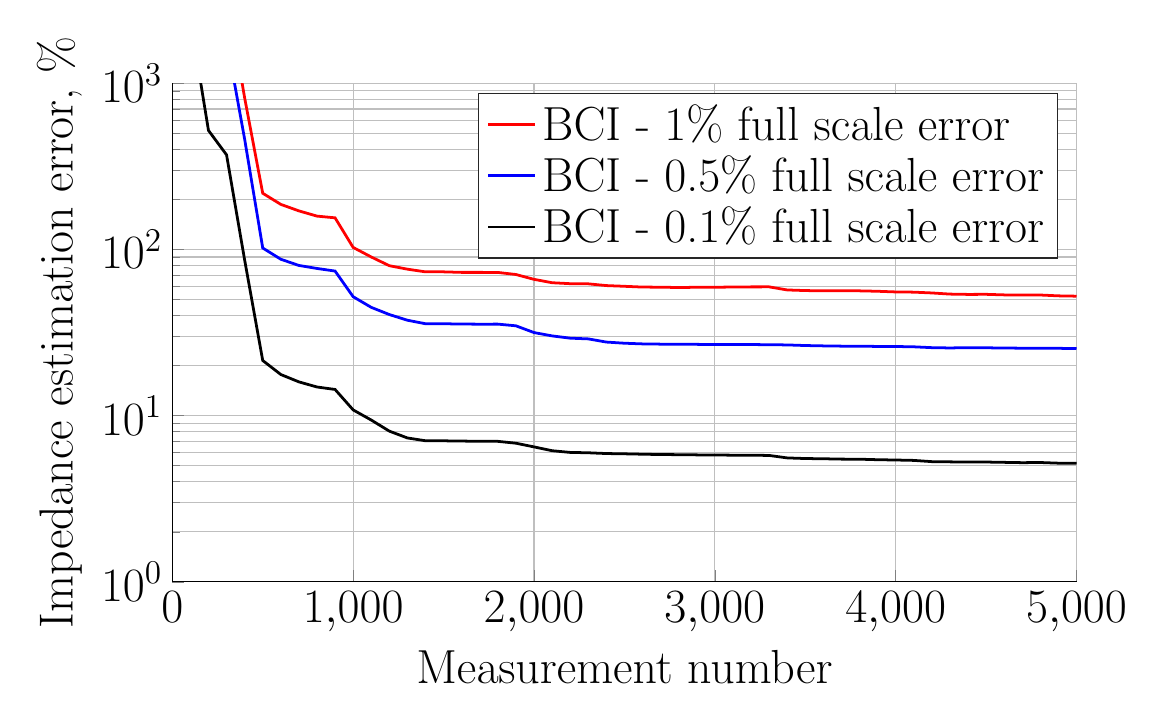
\begin{tikzpicture}

\begin{axis}[%
width=4.521in,
height=2.493in,
at={(0.758in,0.434in)},
scale only axis,
xmin=0,
xmax=5000,
xtick={   0, 1000, 2000, 3000, 4000, 5000},
xlabel={Measurement number},
xmajorgrids,
ymode=log,
ymin=1,
ymax=1000,
yminorticks=true,
% ylabel={$\frac{\|\mathbf{z} - \hat{\mathbf{z}}\|_2}{\|\mathbf{z}\|_2}$, \%},
ylabel={Impedance estimation error, \%},
ymajorgrids,
yminorgrids,
axis background/.style={fill=white},
axis x line*=bottom,
axis y line*=left,
%legend style={at={(0.5,1.03)},anchor=south,legend cell align=left,align=left,draw=white!15!black},
legend style={legend cell align=left, align=right, draw=white!15!black},
xlabel style={font=\LARGE},ylabel style={font=\LARGE},legend style={font=\LARGE},ticklabel style={font=\LARGE}
]
\addplot [color=red,solid,line width=1.0pt]
  table[row sep=crcr]{%
100	22728.0844401917\\
200	5118.69657000351\\
300	3536.99850914306\\
400	816.769790166386\\
500	217.789962578717\\
600	186.673358272156\\
700	170.588712436484\\
800	158.672266693795\\
900	154.945990194417\\
1000	102.812960987144\\
1100	90.0903675033844\\
1200	79.8235730543928\\
1300	76.0952811801202\\
1400	73.2939001233863\\
1500	73.3105008058256\\
1600	72.7745763727444\\
1700	72.7783815896182\\
1800	72.718031543639\\
1900	70.6605592162223\\
2000	66.0800688049927\\
2100	63.0546347055478\\
2200	62.2194878973759\\
2300	62.0956124039623\\
2400	60.6097719919569\\
2500	60.0059486729373\\
2600	59.3725361804331\\
2700	59.273596157382\\
2800	58.9970650417395\\
2900	59.2004854022767\\
3000	59.2540643803915\\
3100	59.3824432036232\\
3200	59.5270961745916\\
3300	59.5457679559992\\
3400	57.0456483739896\\
3500	56.5590202126003\\
3600	56.3618548265959\\
3700	56.3310515498867\\
3800	56.3326145456274\\
3900	56.0118499285963\\
4000	55.4987848173866\\
4100	55.3352463267593\\
4200	54.7210962583346\\
4300	53.8589408369959\\
4400	53.6297037181513\\
4500	53.6839536356162\\
4600	53.2751694592901\\
4700	53.2522253135632\\
4800	53.177736128386\\
4900	52.5670815106881\\
5000	52.3268073688193\\
};
\addlegendentry{BCI - 1\% full scale error};

\addplot [color=blue,solid,line width=1.0pt]
  table[row sep=crcr]{%
100	11400.6317104915\\
200	2709.11003762981\\
300	1837.480807797\\
400	460.735052239631\\
500	102.005394167206\\
600	87.2906130185545\\
700	80.0915493937165\\
800	76.8472619532403\\
900	74.1173835937968\\
1000	51.9491088048463\\
1100	44.8245611687652\\
1200	40.5784875779692\\
1300	37.5024040866603\\
1400	35.7216733221953\\
1500	35.7193452101075\\
1600	35.5593681721333\\
1700	35.5168223438536\\
1800	35.5311590526479\\
1900	34.7140095542001\\
2000	31.6135326665586\\
2100	30.1820496229043\\
2200	29.251150624789\\
2300	28.9584491275208\\
2400	27.7120685560186\\
2500	27.2715114539494\\
2600	27.0170947009927\\
2700	26.9242291975569\\
2800	26.8678826767531\\
2900	26.8440375438859\\
3000	26.772186808124\\
3100	26.7609659888137\\
3200	26.7669739770353\\
3300	26.7189769781261\\
3400	26.6314209655037\\
3500	26.4145706764439\\
3600	26.281180847016\\
3700	26.18937750428\\
3800	26.1581314055083\\
3900	26.086201997588\\
4000	26.0601240884831\\
4100	25.9459986670809\\
4200	25.6442362748963\\
4300	25.5423909233786\\
4400	25.6431195654694\\
4500	25.5931984861965\\
4600	25.5147322817117\\
4700	25.4599795184458\\
4800	25.4167488602764\\
4900	25.4113724076065\\
5000	25.3137359321453\\
};
\addlegendentry{BCI - 0.5\% full scale error};

\addplot [color=black,solid,line width=1.0pt]
  table[row sep=crcr]{%
100	2426.97935227751\\
200	520.097429495387\\
300	370.627433664178\\
400	86.4088147076159\\
500	21.4660738897338\\
600	17.6791178477347\\
700	15.9634979839217\\
800	14.8705928411826\\
900	14.3726130409558\\
1000	10.8271106697378\\
1100	9.40872402129834\\
1200	8.06864024640509\\
1300	7.34031789104499\\
1400	7.06138614146183\\
1500	7.05484216150573\\
1600	7.0294981712566\\
1700	7.01212772537375\\
1800	7.00416054756797\\
1900	6.82498779889169\\
2000	6.48510124758661\\
2100	6.15065684701161\\
2200	6.00827285737952\\
2300	5.97754929288951\\
2400	5.9144943049684\\
2500	5.89186642858549\\
2600	5.85979970044402\\
2700	5.83257088974041\\
2800	5.82381641579081\\
2900	5.8059225153119\\
3000	5.79328015943364\\
3100	5.78378652643428\\
3200	5.778141003319\\
3300	5.76138406166361\\
3400	5.56721982716132\\
3500	5.51920557437916\\
3600	5.50204025657614\\
3700	5.47477625359662\\
3800	5.46857327003434\\
3900	5.43009535981615\\
4000	5.40738490087627\\
4100	5.37831097108823\\
4200	5.28639416421409\\
4300	5.27038746815866\\
4400	5.2594982138701\\
4500	5.25765191351608\\
4600	5.23462274053984\\
4700	5.2121104596335\\
4800	5.22313758218916\\
4900	5.1755789476994\\
5000	5.1637319100943\\
};
\addlegendentry{BCI - 0.1\% full scale error};

\end{axis}
\end{tikzpicture}%
% \end{document}
			\end{adjustbox}
		\end{column}
		\begin{column}{0.55\textwidth}
			\centering
			\begin{adjustbox}{width=1\columnwidth}
			% This file was created by matlab2tikz.
%
%The latest updates can be retrieved from
%  http://www.mathworks.com/matlabcentral/fileexchange/22022-matlab2tikz-matlab2tikz
%where you can also make suggestions and rate matlab2tikz.
%
\documentclass[tikz]{standalone}
\usepackage[T1]{fontenc}
\usepackage[utf8]{inputenc}
\usepackage{pgfplots}
\usepackage{grffile}
\pgfplotsset{compat=newest}
\usetikzlibrary{plotmarks}
\usepgfplotslibrary{patchplots}
\usepackage{amsmath}

\begin{document}
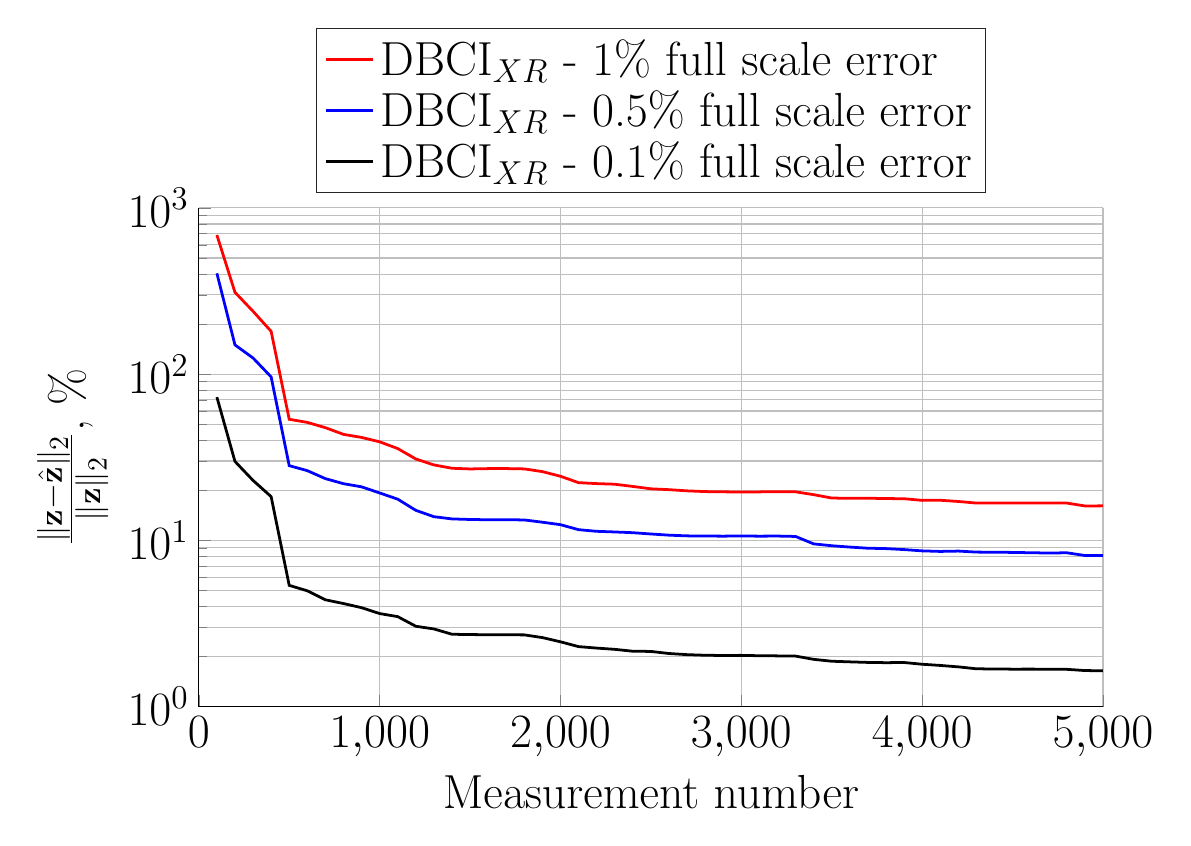
\begin{tikzpicture}

\begin{axis}[%
width=4.521in,
height=2.493in,
at={(0.758in,0.434in)},
scale only axis,
xmin=0,
xmax=5000,
xtick={   0, 1000, 2000, 3000, 4000, 5000},
xlabel={Measurement number},
xmajorgrids,
ymode=log,
ymin=1,
ymax=1000,
yminorticks=true,
ylabel={$\frac{\|\mathbf{z} - \hat{\mathbf{z}}\|_2}{\|\mathbf{z}\|_2}$, \%},
ymajorgrids,
yminorgrids,
axis background/.style={fill=white},
axis x line*=bottom,
axis y line*=left,
legend style={at={(0.5,1.03)},anchor=south,legend cell align=left,align=left,draw=white!15!black},
xlabel style={font=\LARGE},ylabel style={font=\LARGE},legend style={font=\LARGE},ticklabel style={font=\LARGE}
]

\addplot [color=red,solid,line width=1.0pt]
  table[row sep=crcr]{%
100	687.162632312096\\
200	310.581909851338\\
300	238.8564667258\\
400	180.902080862412\\
500	53.4955991216033\\
600	51.2362052694262\\
700	47.625529793001\\
800	43.4151969883932\\
900	41.6042688251828\\
1000	39.1592652954947\\
1100	35.6674632497747\\
1200	30.8666349120025\\
1300	28.4308514040445\\
1400	27.1421605790363\\
1500	26.8893304853057\\
1600	27.0088309173177\\
1700	27.0210911435296\\
1800	26.9021906597949\\
1900	25.909629026642\\
2000	24.2939280348576\\
2100	22.2330831591075\\
2200	21.9430333743929\\
2300	21.7602911615194\\
2400	21.0996757855984\\
2500	20.4152038530171\\
2600	20.1781764715397\\
2700	19.8531190698737\\
2800	19.6471796084147\\
2900	19.5783091473384\\
3000	19.5478853043168\\
3100	19.5685040159804\\
3200	19.6250956269494\\
3300	19.5835760920241\\
3400	18.8266934184721\\
3500	17.9666396640691\\
3600	17.9064595928047\\
3700	17.9216792159022\\
3800	17.8410373739834\\
3900	17.7969598729175\\
4000	17.3979067603842\\
4100	17.4239973806169\\
4200	17.1328370985482\\
4300	16.7613593265288\\
4400	16.7802145012919\\
4500	16.7797938421224\\
4600	16.7930000447739\\
4700	16.7899473869768\\
4800	16.7567820457399\\
4900	16.1031637272547\\
5000	16.1241967612528\\
};
\addlegendentry{DBCI$_{XR}$ - 1\% full scale error};

\addplot [color=blue,solid,line width=1.0pt]
  table[row sep=crcr]{%
100	404.1321725797\\
200	149.907145372373\\
300	125.047013550393\\
400	96.2052957147922\\
500	28.1385540829226\\
600	26.2564948383921\\
700	23.5119455154061\\
800	21.9201928831837\\
900	20.9847690368135\\
1000	19.282089588279\\
1100	17.6908447294148\\
1200	15.1549445078433\\
1300	13.8749438847117\\
1400	13.4550865853242\\
1500	13.3511605321021\\
1600	13.2977969667917\\
1700	13.3066388691057\\
1800	13.2644462935719\\
1900	12.8539181640328\\
2000	12.4206026227885\\
2100	11.5917373605801\\
2200	11.3306951547318\\
2300	11.2297673687889\\
2400	11.1164398891805\\
2500	10.9186750128686\\
2600	10.7415289122971\\
2700	10.6389535941284\\
2800	10.6098105589105\\
2900	10.5977162124967\\
3000	10.6166732692131\\
3100	10.5963378544181\\
3200	10.6086783421659\\
3300	10.5527427481681\\
3400	9.51993532860792\\
3500	9.27804611209175\\
3600	9.10848054090651\\
3700	8.96508734171332\\
3800	8.91796616030325\\
3900	8.79864730528896\\
4000	8.64131244856672\\
4100	8.5756305258051\\
4200	8.61643132577958\\
4300	8.49587863563992\\
4400	8.48170845152912\\
4500	8.45965768252504\\
4600	8.42125014536799\\
4700	8.38815775564816\\
4800	8.41531848948757\\
4900	8.10499014595432\\
5000	8.0932767770725\\
};
\addlegendentry{DBCI$_{XR}$ - 0.5\% full scale error};

\addplot [color=black,solid,line width=1.0pt]
  table[row sep=crcr]{%
100	72.7195490887134\\
200	29.8355381810924\\
300	22.9326955663768\\
400	18.3217119954536\\
500	5.35976617652142\\
600	4.9693423911885\\
700	4.38776740234361\\
800	4.16555527409481\\
900	3.93519315037906\\
1000	3.62564767137419\\
1100	3.47519256870061\\
1200	3.04084066537432\\
1300	2.93004121813041\\
1400	2.72205052231501\\
1500	2.70965158616435\\
1600	2.70543137930573\\
1700	2.70071097718423\\
1800	2.69858839141467\\
1900	2.59940062923238\\
2000	2.45141671070456\\
2100	2.2937077370773\\
2200	2.24764004009169\\
2300	2.20854708761487\\
2400	2.1515491404239\\
2500	2.14573839185848\\
2600	2.08475565438333\\
2700	2.05198197165185\\
2800	2.03458243419119\\
2900	2.02860411526808\\
3000	2.03171625846985\\
3100	2.02131144427194\\
3200	2.01716151247194\\
3300	2.01121763815109\\
3400	1.9230171551157\\
3500	1.87301500214421\\
3600	1.85730571413849\\
3700	1.84271459294255\\
3800	1.83633521278918\\
3900	1.84035199739431\\
4000	1.79664021587933\\
4100	1.76738193462632\\
4200	1.73275273990007\\
4300	1.68679283100553\\
4400	1.68237342382349\\
4500	1.67865029296265\\
4600	1.67946483079034\\
4700	1.6775715993085\\
4800	1.67466385165876\\
4900	1.64625904730214\\
5000	1.64095509018859\\
};
\addlegendentry{DBCI$_{XR}$ - 0.1\% full scale error};

\end{axis}
\end{tikzpicture}%
\end{document}
			\end{adjustbox}
		\end{column}
		\end{columns}
	}

\end{column}

\end{columns}

\end{frame}




\begin{frame}[t]{Simulation results. Long power lines}

\begin{columns}[t]
\begin{column}{0.4\textwidth}
\centering
\begin{itemize}
\item Linear feeder
\item 10 loads
\item Length of power lines: $1-2$km
\item European LV Test Feeder data
\item Noise: 
	\begin{itemize}
		\item Gaussian, full scale
	\end{itemize}
\item Algorithms:
	\begin{itemize}
		\item BCI - original
	\end{itemize}
\item Result:
	\begin{itemize}
		\item \textbf{2-5} times better accuracy
	\end{itemize}
\end{itemize}
\end{column}
\begin{column}{0.7\textwidth}
	\textbf{Note}: LBCI performance is equivalent to that of conventional approaches
	\centering
	\begin{figure}[H]
	\begin{adjustbox}{width=0.75\columnwidth}
	% This file was created by matlab2tikz.
%
%The latest updates can be retrieved from
%  http://www.mathworks.com/matlabcentral/fileexchange/22022-matlab2tikz-matlab2tikz
%where you can also make suggestions and rate matlab2tikz.
%
% \documentclass[tikz]{standalone}
% \usepackage[T1]{fontenc}
% \usepackage[utf8]{inputenc}
% \usepackage{pgfplots}
% \usepackage{grffile}
% \pgfplotsset{compat=newest}
% \usetikzlibrary{plotmarks}
% \usepgfplotslibrary{patchplots}
% \usepackage{amsmath}

% \begin{document}
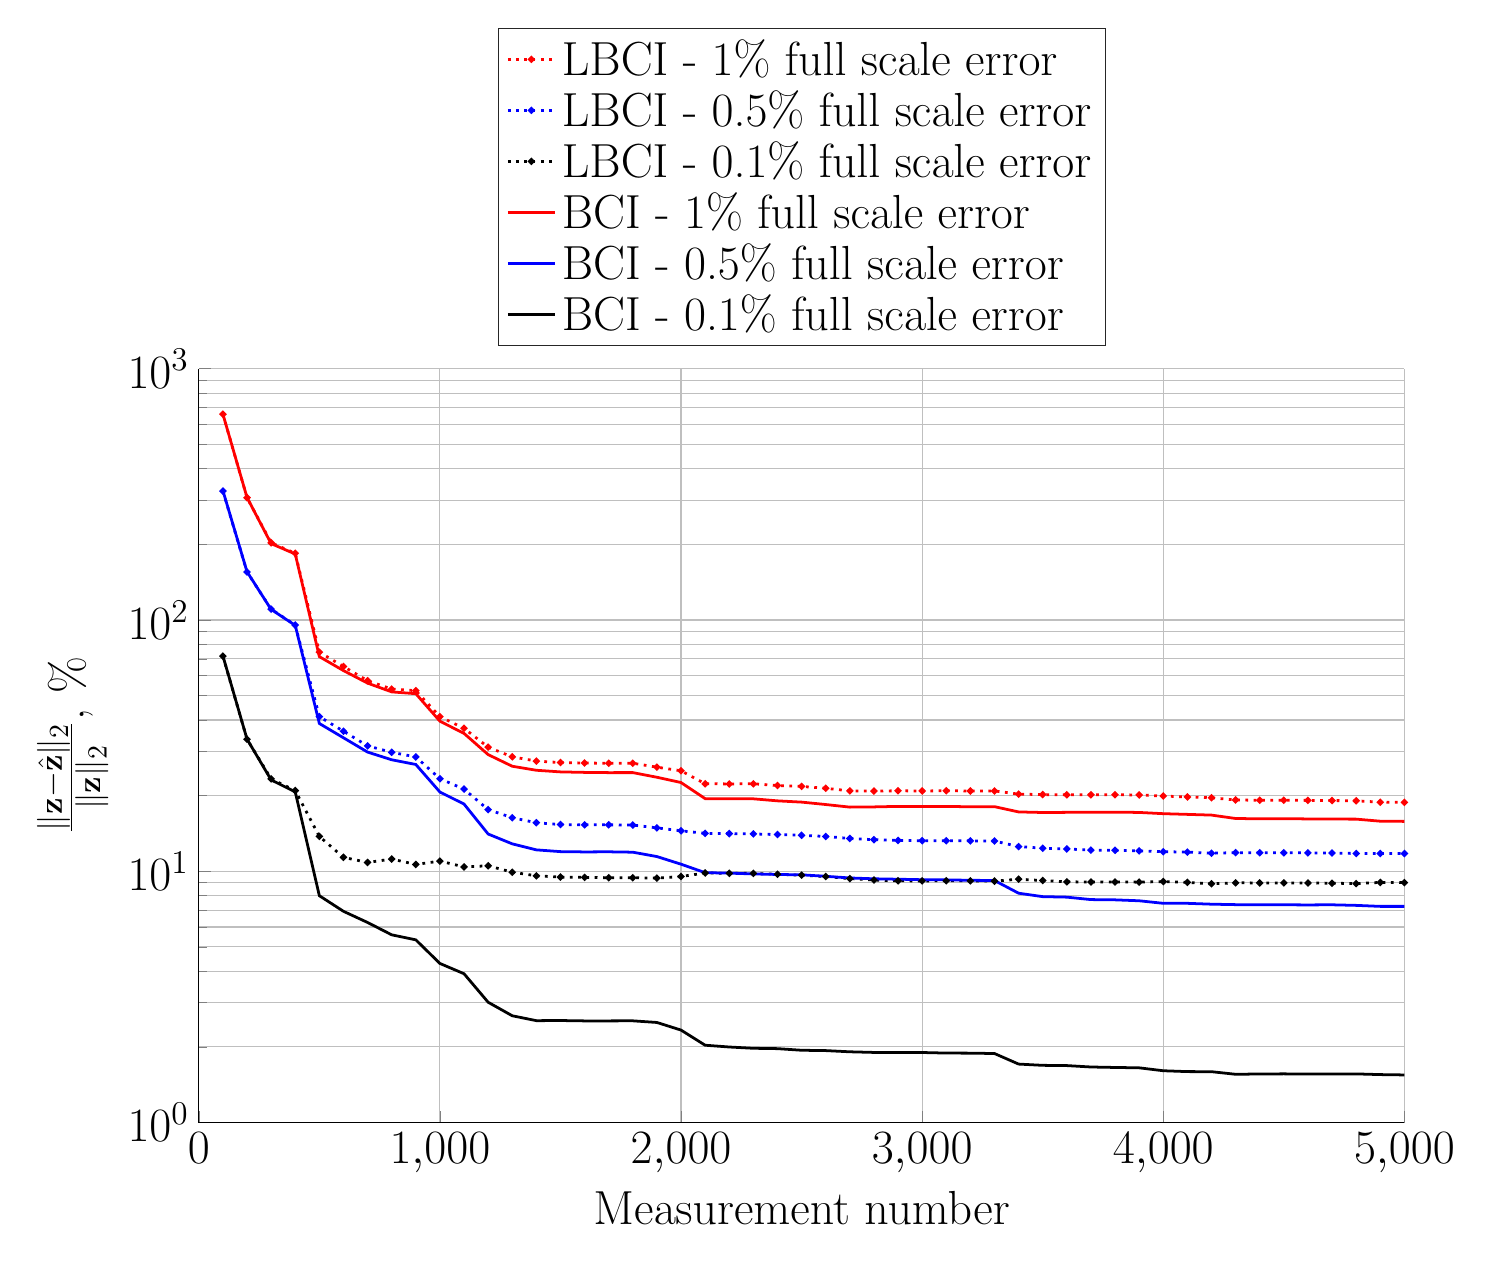
\begin{tikzpicture}

\begin{axis}[%
width=6.028in,
height=3.769in,
at={(1.011in,0.509in)},
scale only axis,
xmin=0,
xmax=5000,
xtick={   0, 1000, 2000, 3000, 4000, 5000},
xlabel={Measurement number},
xmajorgrids,
ymode=log,
ymin=1,
ymax=1000,
yminorticks=true,
ylabel={$\frac{\|\mathbf{z} - \hat{\mathbf{z}}\|_2}{\|\mathbf{z}\|_2}$, \%},
ymajorgrids,
yminorgrids,
axis background/.style={fill=white},
axis x line*=bottom,
axis y line*=left,
legend style={at={(0.5,1.03)},anchor=south,legend cell align=left,align=left,draw=white!15!black},
xlabel style={font=\LARGE},ylabel style={font=\LARGE},legend style={font=\LARGE},ticklabel style={font=\LARGE}
]
\addplot [color=red,dotted,line width=1.0pt,mark size=0.7pt,mark=*,mark options={solid}]
  table[row sep=crcr]{%
100	659.040534857702\\
200	306.80206106422\\
300	202.922606522803\\
400	184.27915420211\\
500	74.4704195738183\\
600	65.302035719461\\
700	57.3290890863622\\
800	53.0782732352832\\
900	52.323212175496\\
1000	41.2297135264796\\
1100	37.06800933764\\
1200	31.1708657492995\\
1300	28.5307090304024\\
1400	27.44627439343\\
1500	27.0745167846451\\
1600	26.9631606437801\\
1700	26.8984670467172\\
1800	26.9084358644316\\
1900	25.9551686685729\\
2000	25.108726644597\\
2100	22.2956337843983\\
2200	22.2633406784104\\
2300	22.2916275857289\\
2400	21.9397445129273\\
2500	21.7571665685396\\
2600	21.3864445891304\\
2700	20.8868182867011\\
2800	20.8551033191808\\
2900	20.9010994549578\\
3000	20.8686650046051\\
3100	20.9124703000949\\
3200	20.8649528940537\\
3300	20.879100147923\\
3400	20.2736837839125\\
3500	20.1870360368623\\
3600	20.1483733715194\\
3700	20.1434208685339\\
3800	20.1541992817378\\
3900	20.120723953138\\
4000	19.9277625715534\\
4100	19.7542004915796\\
4200	19.6090014861816\\
4300	19.2160115690463\\
4400	19.1669184580374\\
4500	19.1719221538792\\
4600	19.1452710662481\\
4700	19.1159603514197\\
4800	19.0748744457345\\
4900	18.8335536134415\\
5000	18.8003659417871\\
};
\addlegendentry{LBCI - 1\% full scale error};

\addplot [color=blue,dotted,line width=1.0pt,mark size=0.7pt,mark=*,mark options={solid}]
  table[row sep=crcr]{%
100	325.939763095285\\
200	155.305033657335\\
300	110.411672317769\\
400	95.4146877978017\\
500	41.249436770124\\
600	36.0799825249198\\
700	31.5515105083569\\
800	29.7407468237229\\
900	28.5139786412904\\
1000	23.3469491449701\\
1100	21.2283873729015\\
1200	17.5892945136175\\
1300	16.3329394225103\\
1400	15.5986178330847\\
1500	15.3392836535708\\
1600	15.3030886303937\\
1700	15.3013568747385\\
1800	15.2723262564557\\
1900	14.8839722243997\\
2000	14.4851641842197\\
2100	14.1518047703867\\
2200	14.1183832560406\\
2300	14.0758549689415\\
2400	13.9949994416347\\
2500	13.9070829485743\\
2600	13.7552356520581\\
2700	13.505073096113\\
2800	13.3534689842058\\
2900	13.2658197596707\\
3000	13.2278015007836\\
3100	13.2300607379895\\
3200	13.2102023486308\\
3300	13.186987940092\\
3400	12.5409473242492\\
3500	12.3511909319057\\
3600	12.26799573637\\
3700	12.1353927885668\\
3800	12.1142811230124\\
3900	12.0523914594524\\
4000	11.9651291018913\\
4100	11.9173615199099\\
4200	11.7982989393014\\
4300	11.8609818939798\\
4400	11.8495505040594\\
4500	11.8453263970241\\
4600	11.8344695876821\\
4700	11.8186064625387\\
4800	11.7672816465301\\
4900	11.7743649326105\\
5000	11.7632499127752\\
};
\addlegendentry{LBCI - 0.5\% full scale error};

\addplot [color=black,dotted,line width=1.0pt,mark size=0.7pt,mark=*,mark options={solid}]
  table[row sep=crcr]{%
100	71.8022323347998\\
200	33.5281508422428\\
300	23.3159265416903\\
400	20.9351102185999\\
500	13.7629070258335\\
600	11.358207818472\\
700	10.8396584874401\\
800	11.1827066979431\\
900	10.6439571015401\\
1000	10.9752048229656\\
1100	10.4062099477565\\
1200	10.5142233534481\\
1300	9.91349750262337\\
1400	9.59147621152229\\
1500	9.47820241714138\\
1600	9.45209137703198\\
1700	9.42662008795498\\
1800	9.41885346762396\\
1900	9.3923495929566\\
2000	9.52883194479701\\
2100	9.84218757470693\\
2200	9.80857438950287\\
2300	9.80742495264447\\
2400	9.72782068631855\\
2500	9.6449617653382\\
2600	9.53036152927272\\
2700	9.3478429288162\\
2800	9.22839299045763\\
2900	9.1612579858623\\
3000	9.15255463183914\\
3100	9.16315026376884\\
3200	9.16010683777694\\
3300	9.13424602543443\\
3400	9.29776501168745\\
3500	9.18245897227697\\
3600	9.07642578779062\\
3700	9.0649821038938\\
3800	9.06338048113857\\
3900	9.05060245662827\\
4000	9.09696308306439\\
4100	9.02984178062694\\
4200	8.91456351897199\\
4300	8.99263264164221\\
4400	8.98700538504772\\
4500	8.98781087357142\\
4600	8.98245974680313\\
4700	8.96250748953804\\
4800	8.93097907012001\\
4900	9.02799943896461\\
5000	9.00963044088909\\
};
\addlegendentry{LBCI - 0.1\% full scale error};

\addplot [color=red,solid,line width=1.0pt]
  table[row sep=crcr]{%
100	659.56881658749\\
200	307.301241447016\\
300	201.32307985644\\
400	183.048146929529\\
500	71.4734203225816\\
600	62.8829862479565\\
700	56.0648964454405\\
800	51.7403645671444\\
900	50.8909332085476\\
1000	39.5480465087212\\
1100	35.3693373314896\\
1200	29.1246375562055\\
1300	26.1757073825054\\
1400	25.2293016732408\\
1500	24.8535576227902\\
1600	24.742855389003\\
1700	24.6866695156716\\
1800	24.6919392958537\\
1900	23.6626260819765\\
2000	22.5470417196135\\
2100	19.456433102685\\
2200	19.4338467039465\\
2300	19.4249202277284\\
2400	19.0647680565012\\
2500	18.8452931322232\\
2600	18.4315363725663\\
2700	17.998981725382\\
2800	18.0342982314189\\
2900	18.1199328673537\\
3000	18.0830753664742\\
3100	18.1088959258068\\
3200	18.0591309631655\\
3300	18.0740087008344\\
3400	17.2248911077859\\
3500	17.1330901203646\\
3600	17.1559751066928\\
3700	17.1881760649542\\
3800	17.1892395968817\\
3900	17.1431805387667\\
4000	16.9495792721079\\
4100	16.8409564873455\\
4200	16.7311388506264\\
4300	16.2190677222075\\
4400	16.1692003673591\\
4500	16.1819692862289\\
4600	16.1554878603417\\
4700	16.1310605934899\\
4800	16.1226976603156\\
4900	15.8201195044776\\
5000	15.7940658119176\\
};
\addlegendentry{BCI - 1\% full scale error};

\addplot [color=blue,solid,line width=1.0pt]
  table[row sep=crcr]{%
100	327.111291797483\\
200	155.631950217755\\
300	110.152025521629\\
400	95.1843497018664\\
500	38.7358972183351\\
600	33.9790764486301\\
700	29.8055176386943\\
800	27.7758985195908\\
900	26.6045603632109\\
1000	20.6658420954446\\
1100	18.5161824556313\\
1200	14.0668412004198\\
1300	12.8532247560692\\
1400	12.1647364321055\\
1500	11.9698602049376\\
1600	11.9378700347329\\
1700	11.9497633267475\\
1800	11.9080679001962\\
1900	11.4411598126037\\
2000	10.6677937860089\\
2100	9.87080049468944\\
2200	9.83105050952715\\
2300	9.75560992404414\\
2400	9.70910135096232\\
2500	9.67797957182692\\
2600	9.54918274226053\\
2700	9.40447390659514\\
2800	9.33203218866336\\
2900	9.29613939549279\\
3000	9.25475556728678\\
3100	9.24050835944374\\
3200	9.20531206054066\\
3300	9.18604070916017\\
3400	8.17666594618074\\
3500	7.92497093708109\\
3600	7.88840505840538\\
3700	7.71424338983087\\
3800	7.69615959142446\\
3900	7.63045170843426\\
4000	7.45434934133202\\
4100	7.45480988173055\\
4200	7.39458664101081\\
4300	7.36457569856779\\
4400	7.35810291141632\\
4500	7.35347974605921\\
4600	7.34662168331193\\
4700	7.35388079006209\\
4800	7.31580144655943\\
4900	7.24861915723705\\
5000	7.24832820182254\\
};
\addlegendentry{BCI - 0.5\% full scale error};

\addplot [color=black,solid,line width=1.0pt]
  table[row sep=crcr]{%
100	71.9541762646144\\
200	33.5714208423819\\
300	23.0963014618009\\
400	20.6938865825754\\
500	7.99384261411036\\
600	6.92782930806457\\
700	6.25376681653603\\
800	5.58500041996704\\
900	5.3338379867869\\
1000	4.29574030341234\\
1100	3.91052795901051\\
1200	3.01098491176513\\
1300	2.66009076324519\\
1400	2.5432381035151\\
1500	2.54630514270835\\
1600	2.53772286418481\\
1700	2.53798012076776\\
1800	2.53935276467103\\
1900	2.50148722650604\\
2000	2.3327724674815\\
2100	2.03064016710436\\
2200	1.99815988831018\\
2300	1.97475963079394\\
2400	1.96831698852112\\
2500	1.9391794510729\\
2600	1.93326065993609\\
2700	1.91211405745849\\
2800	1.9012560051618\\
2900	1.89898745589482\\
3000	1.89969735235255\\
3100	1.88970325620367\\
3200	1.88874581183903\\
3300	1.8820945576694\\
3400	1.70843521121686\\
3500	1.68882991354695\\
3600	1.68490571962326\\
3700	1.66341663541364\\
3800	1.65638371434164\\
3900	1.65086937753352\\
4000	1.60719972069634\\
4100	1.5945916054125\\
4200	1.5933903638057\\
4300	1.55597196508194\\
4400	1.56023326749214\\
4500	1.56199464407532\\
4600	1.55901604396616\\
4700	1.55944716858258\\
4800	1.56132651300968\\
4900	1.55149656017617\\
5000	1.54661416554074\\
};
\addlegendentry{BCI - 0.1\% full scale error};

\end{axis}
\end{tikzpicture}%
\end{document}
	\end{adjustbox}
	\end{figure}
\end{column}
\end{columns}

\end{frame}




\begin{frame}[fragile]{Short questions}

\centering
\includegraphics[scale=0.1]{pics/Question_Mark.png}

\end{frame}


\end{document}